% Auto-generated includegraphics snippets for Bab 4
% Adjust relative path according to your LaTeX project structure.

% fig_4_1_distribusi_label_risiko.png
\begin{figure}[!htbp]
    \centering
    
\includegraphics[width=0.85\textwidth]{fig_4_1_distribusi_label_risiko.png}
    \caption{TODO: sesuaikan caption untuk fig_4_1_distribusi_label_risiko.png}
    \label{fig:fig_4_1_distribusi_label_risiko}
\end{figure}

% fig_4_2_distribusi_label_per_split.png
\begin{figure}[!htbp]
    \centering
    
\includegraphics[width=0.85\textwidth]{fig_4_2_distribusi_label_per_split.png}
    \caption{TODO: sesuaikan caption untuk fig_4_2_distribusi_label_per_split.png}
    \label{fig:fig_4_2_distribusi_label_per_split}
\end{figure}

% fig_4_3_top10_missing_columns.png
\begin{figure}[!htbp]
    \centering
    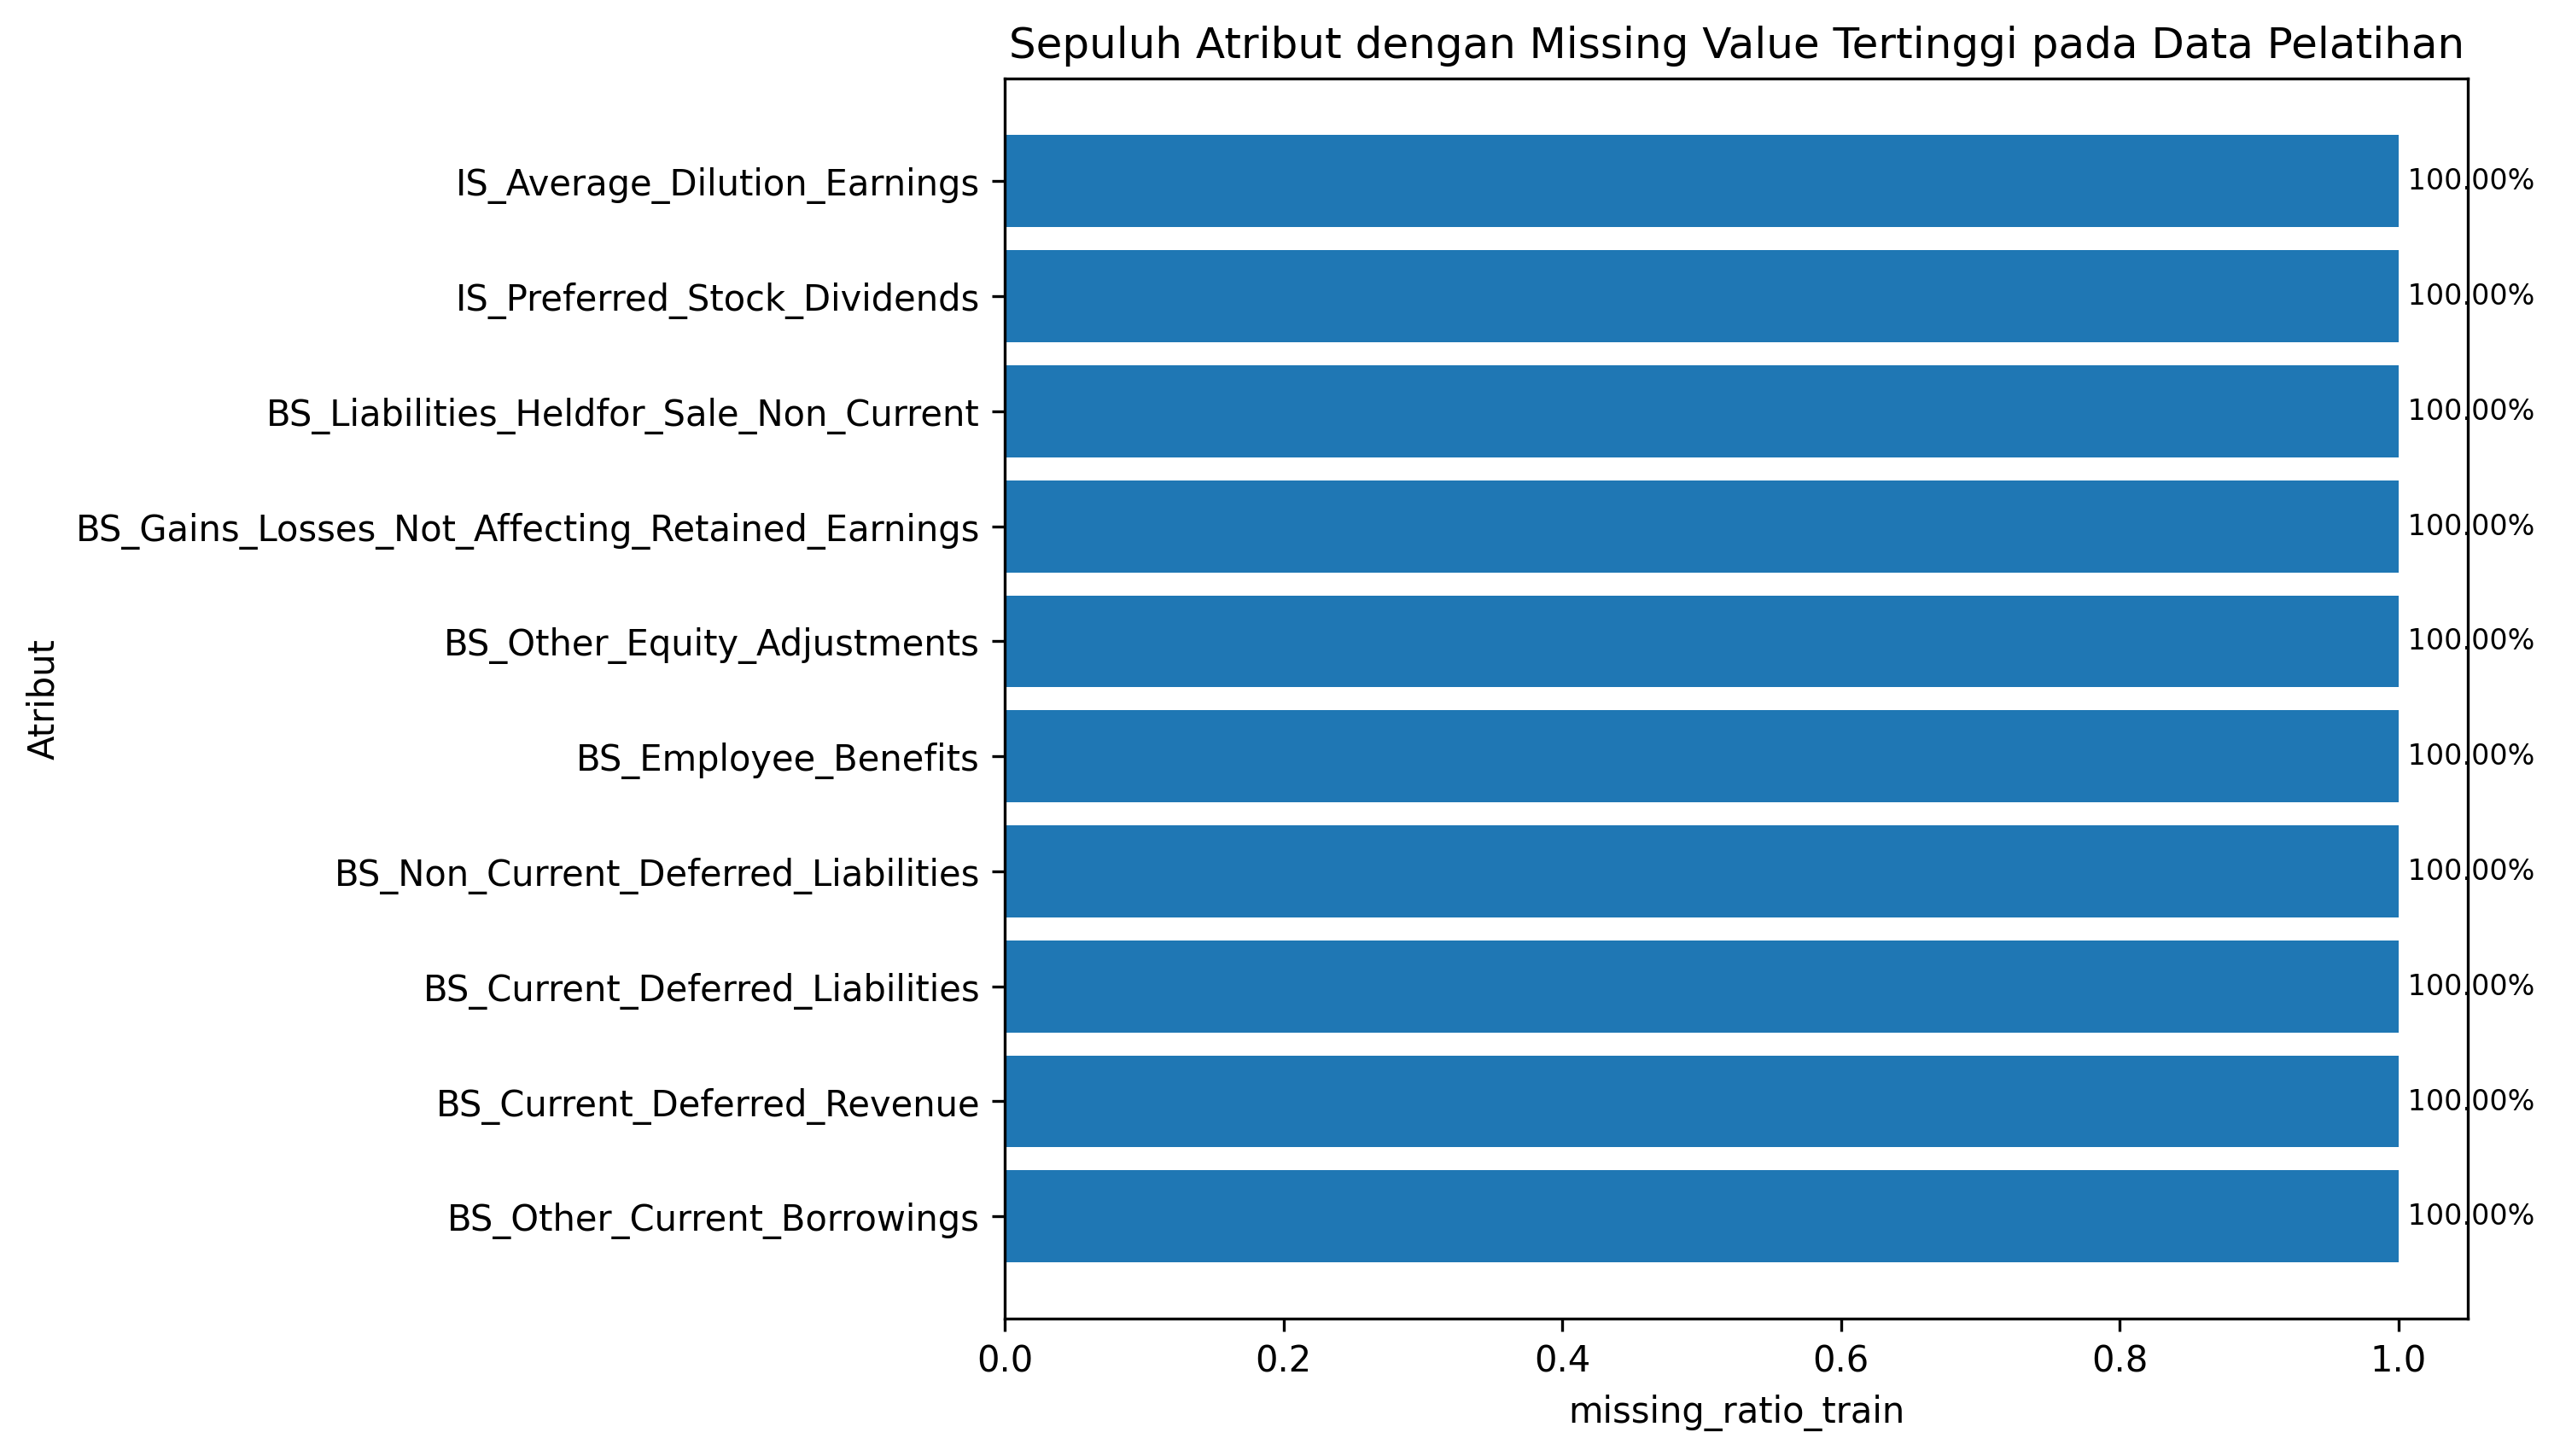
\includegraphics[width=0.85\textwidth]{fig_4_3_top10_missing_columns.png}
    \caption{TODO: sesuaikan caption untuk fig_4_3_top10_missing_columns.png}
    \label{fig:fig_4_3_top10_missing_columns}
\end{figure}

% fig_4_4_perbandingan_kinerja_validasi_model.png
\begin{figure}[!htbp]
    \centering
    
\includegraphics[width=0.85\textwidth]{fig_4_4_perbandingan_kinerja_validasi_model.png}
    \caption{TODO: sesuaikan caption untuk fig_4_4_perbandingan_kinerja_validasi_model.png}
    \label{fig:fig_4_4_perbandingan_kinerja_validasi_model}
\end{figure}

% fig_4_5_cv_vs_macro_f1_validasi.png
\begin{figure}[!htbp]
    \centering
    
\includegraphics[width=0.85\textwidth]{fig_4_5_cv_vs_macro_f1_validasi.png}
    \caption{TODO: sesuaikan caption untuk fig_4_5_cv_vs_macro_f1_validasi.png}
    \label{fig:fig_4_5_cv_vs_macro_f1_validasi}
\end{figure}

% best_model_final_test_confusion_matrix.png
\begin{figure}[!htbp]
    \centering
    
\includegraphics[width=0.85\textwidth]{best_model_final_test_confusion_matrix.png}
    \caption{TODO: sesuaikan caption untuk best_model_final_test_confusion_matrix.png}
    \label{fig:best_model_final_test_confusion_matrix}
\end{figure}

% accuracy_by_certainty_status.png
\begin{figure}[!htbp]
    \centering
    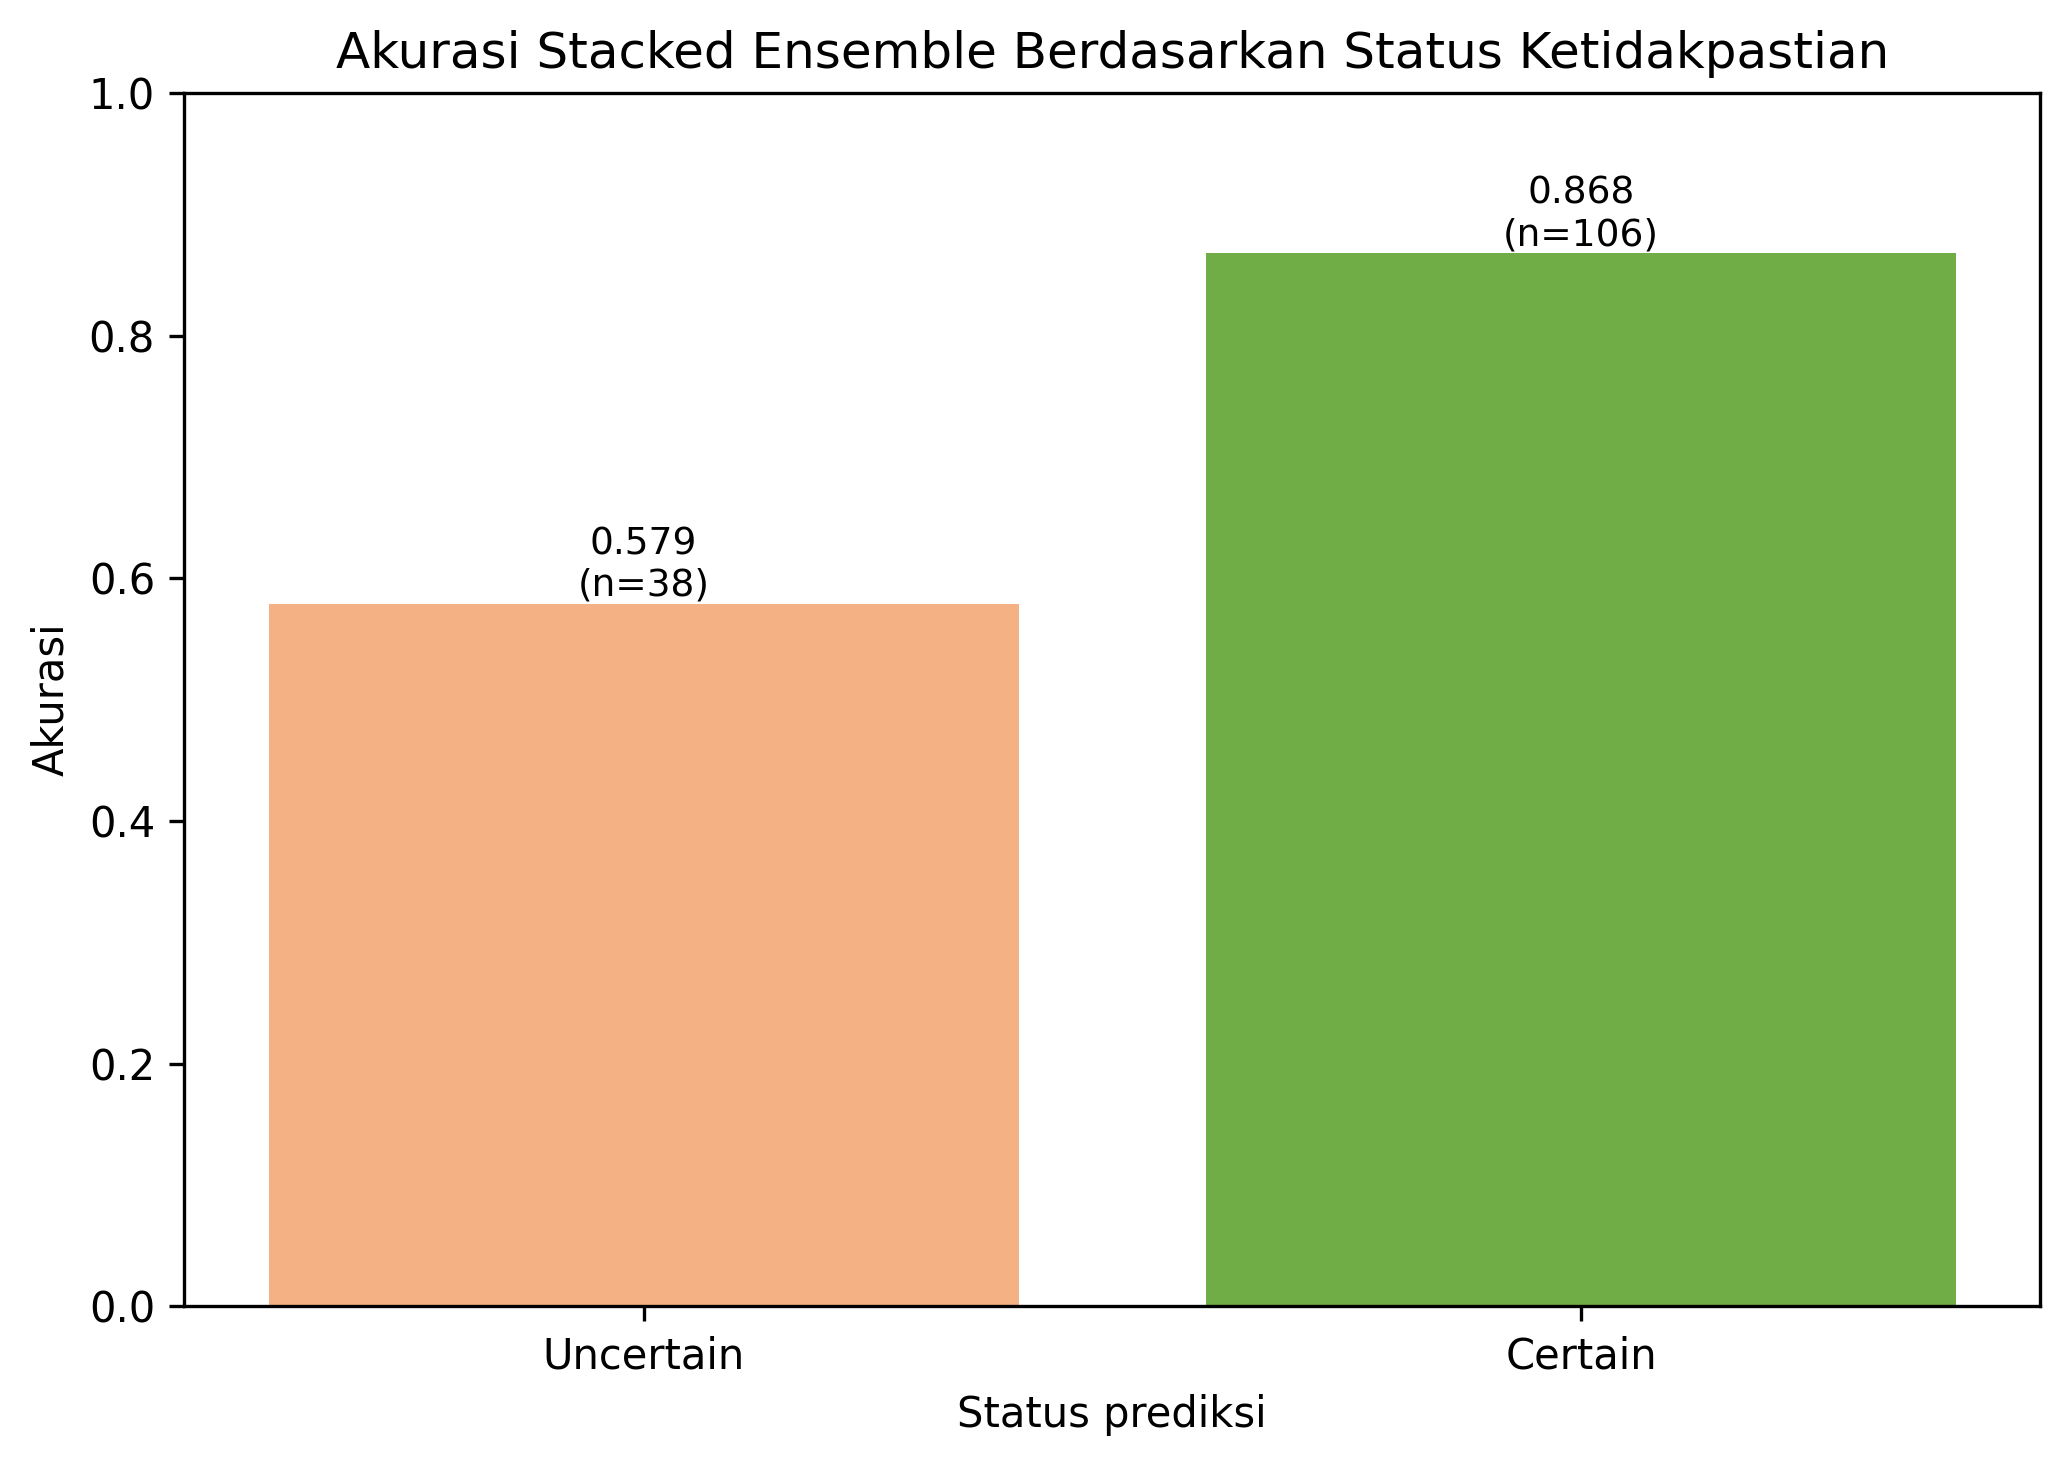
\includegraphics[width=0.85\textwidth]{accuracy_by_certainty_status.png}
    \caption{TODO: sesuaikan caption untuk accuracy_by_certainty_status.png}
    \label{fig:accuracy_by_certainty_status}
\end{figure}

% uncertainty_ratio_by_actual_class.png
\begin{figure}[!htbp]
    \centering
    
\includegraphics[width=0.85\textwidth]{uncertainty_ratio_by_actual_class.png}
    \caption{TODO: sesuaikan caption untuk uncertainty_ratio_by_actual_class.png}
    \label{fig:uncertainty_ratio_by_actual_class}
\end{figure}

% max_probability_distribution.png
\begin{figure}[!htbp]
    \centering
    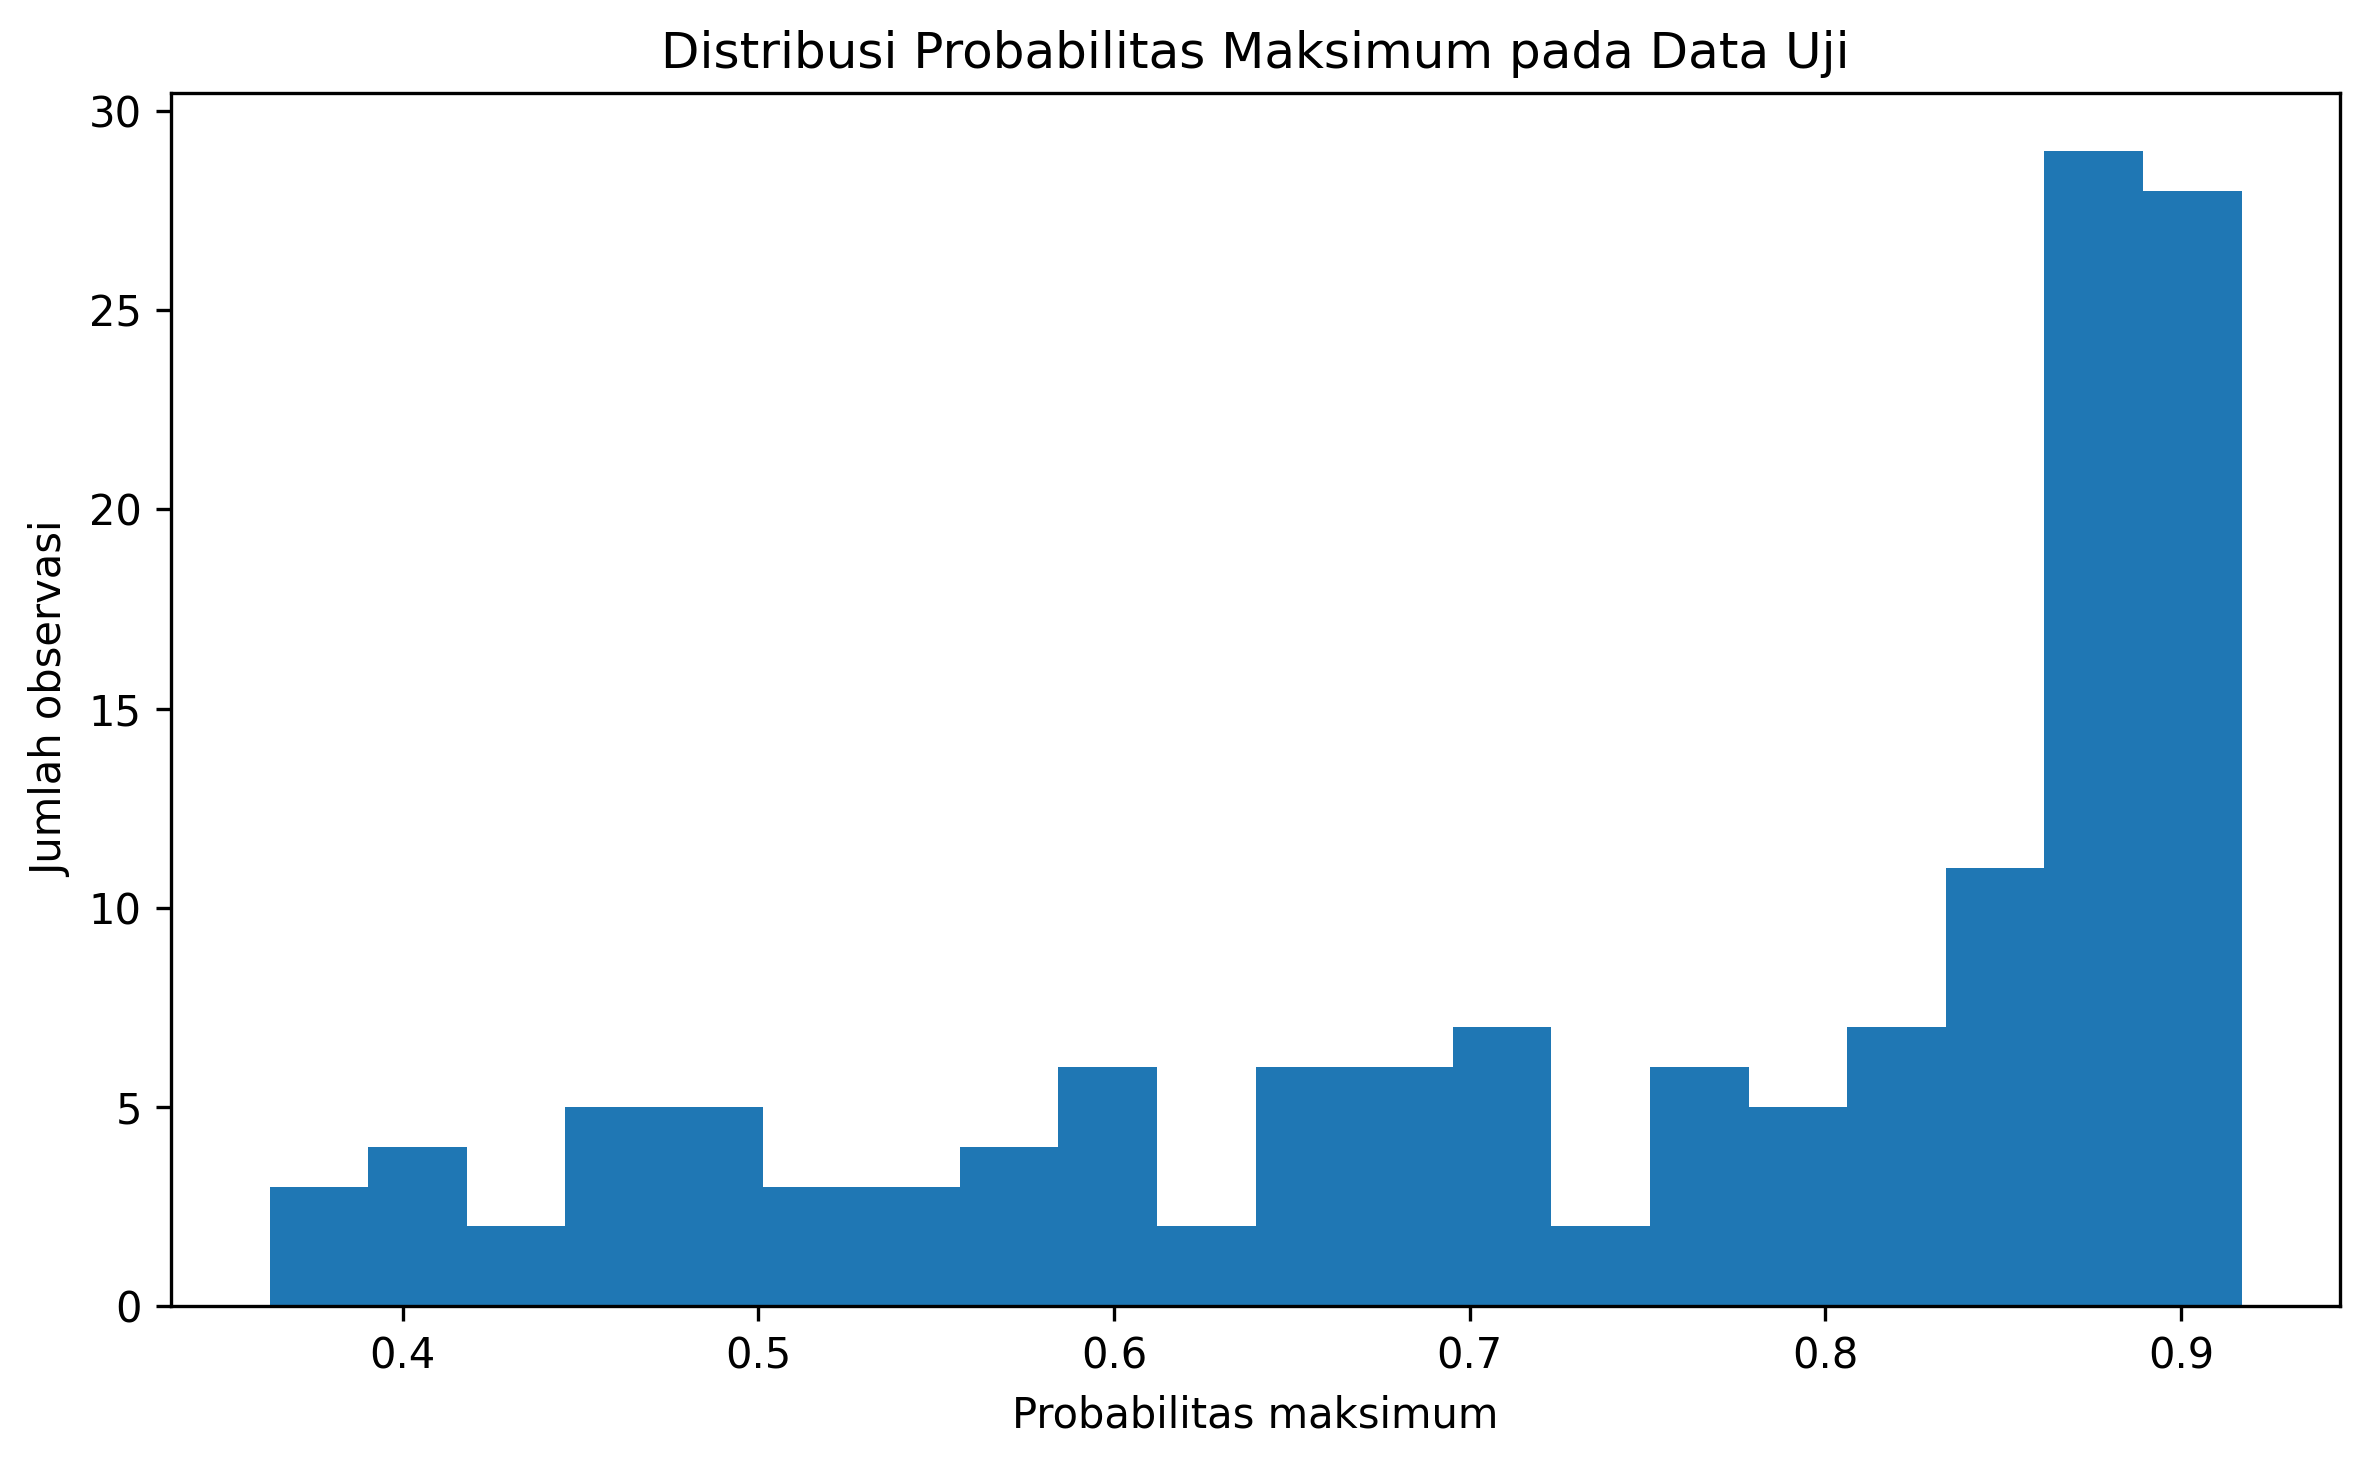
\includegraphics[width=0.85\textwidth]{max_probability_distribution.png}
    \caption{TODO: sesuaikan caption untuk max_probability_distribution.png}
    \label{fig:max_probability_distribution}
\end{figure}

% prediction_margin_distribution.png
\begin{figure}[!htbp]
    \centering
    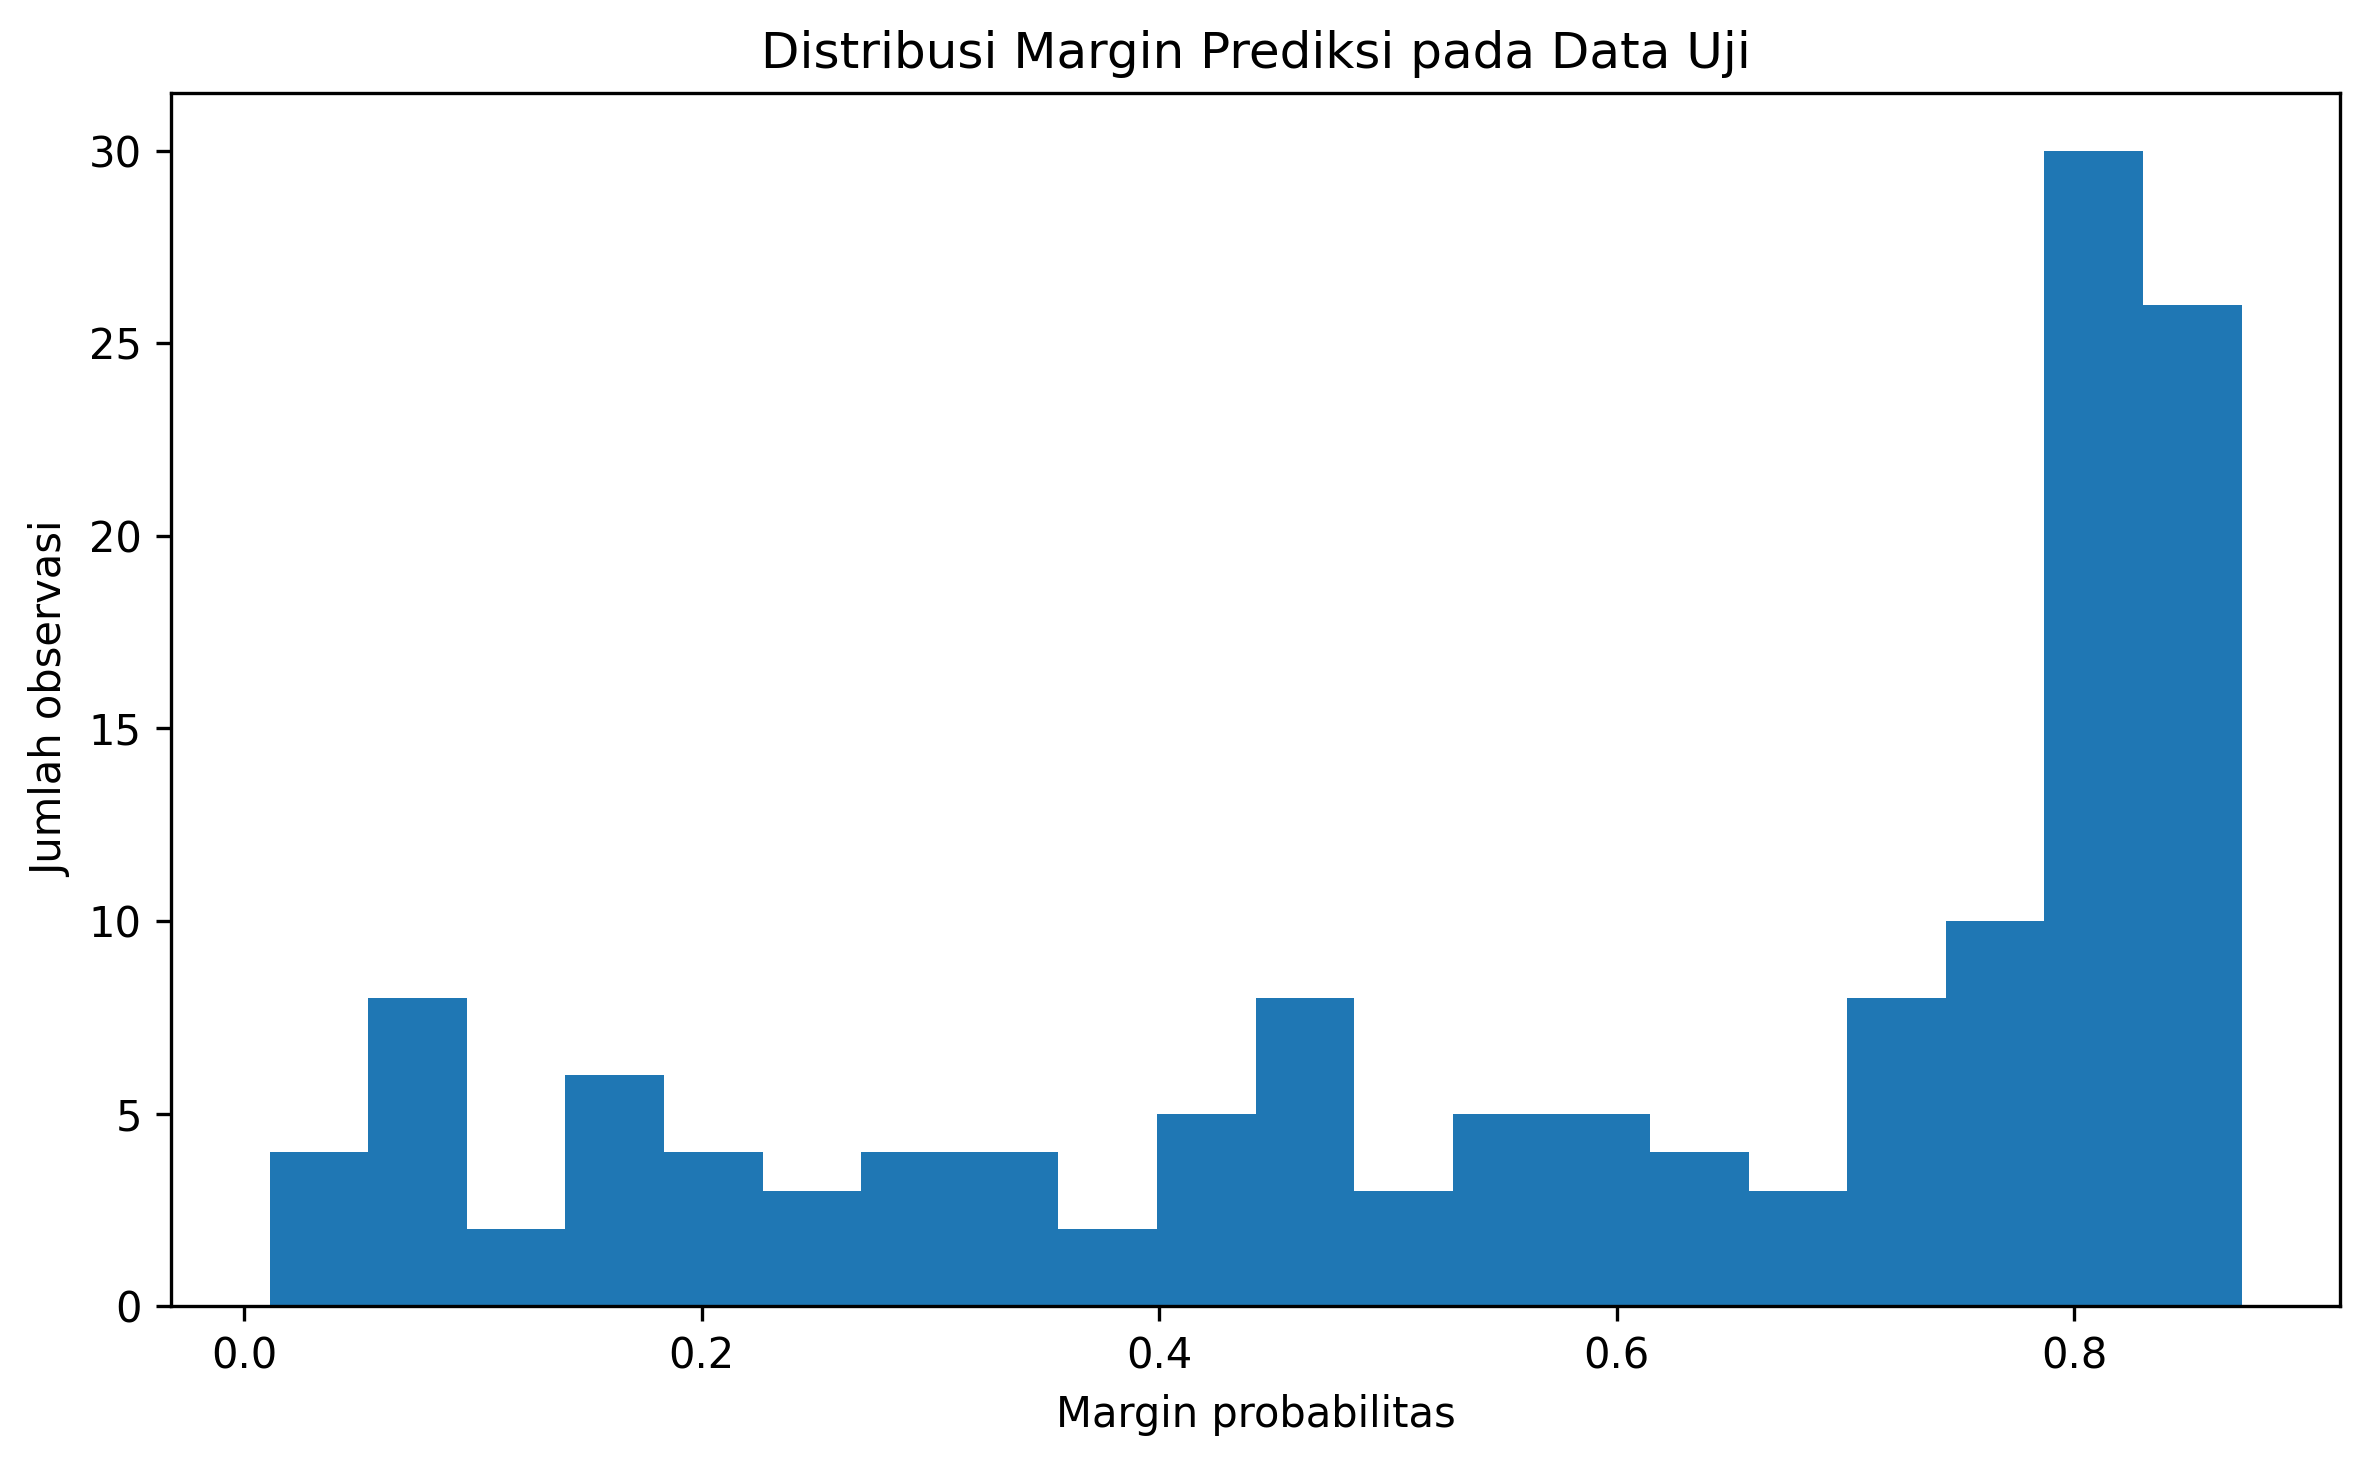
\includegraphics[width=0.85\textwidth]{prediction_margin_distribution.png}
    \caption{TODO: sesuaikan caption untuk prediction_margin_distribution.png}
    \label{fig:prediction_margin_distribution}
\end{figure}

% normalized_entropy_distribution.png
\begin{figure}[!htbp]
    \centering
    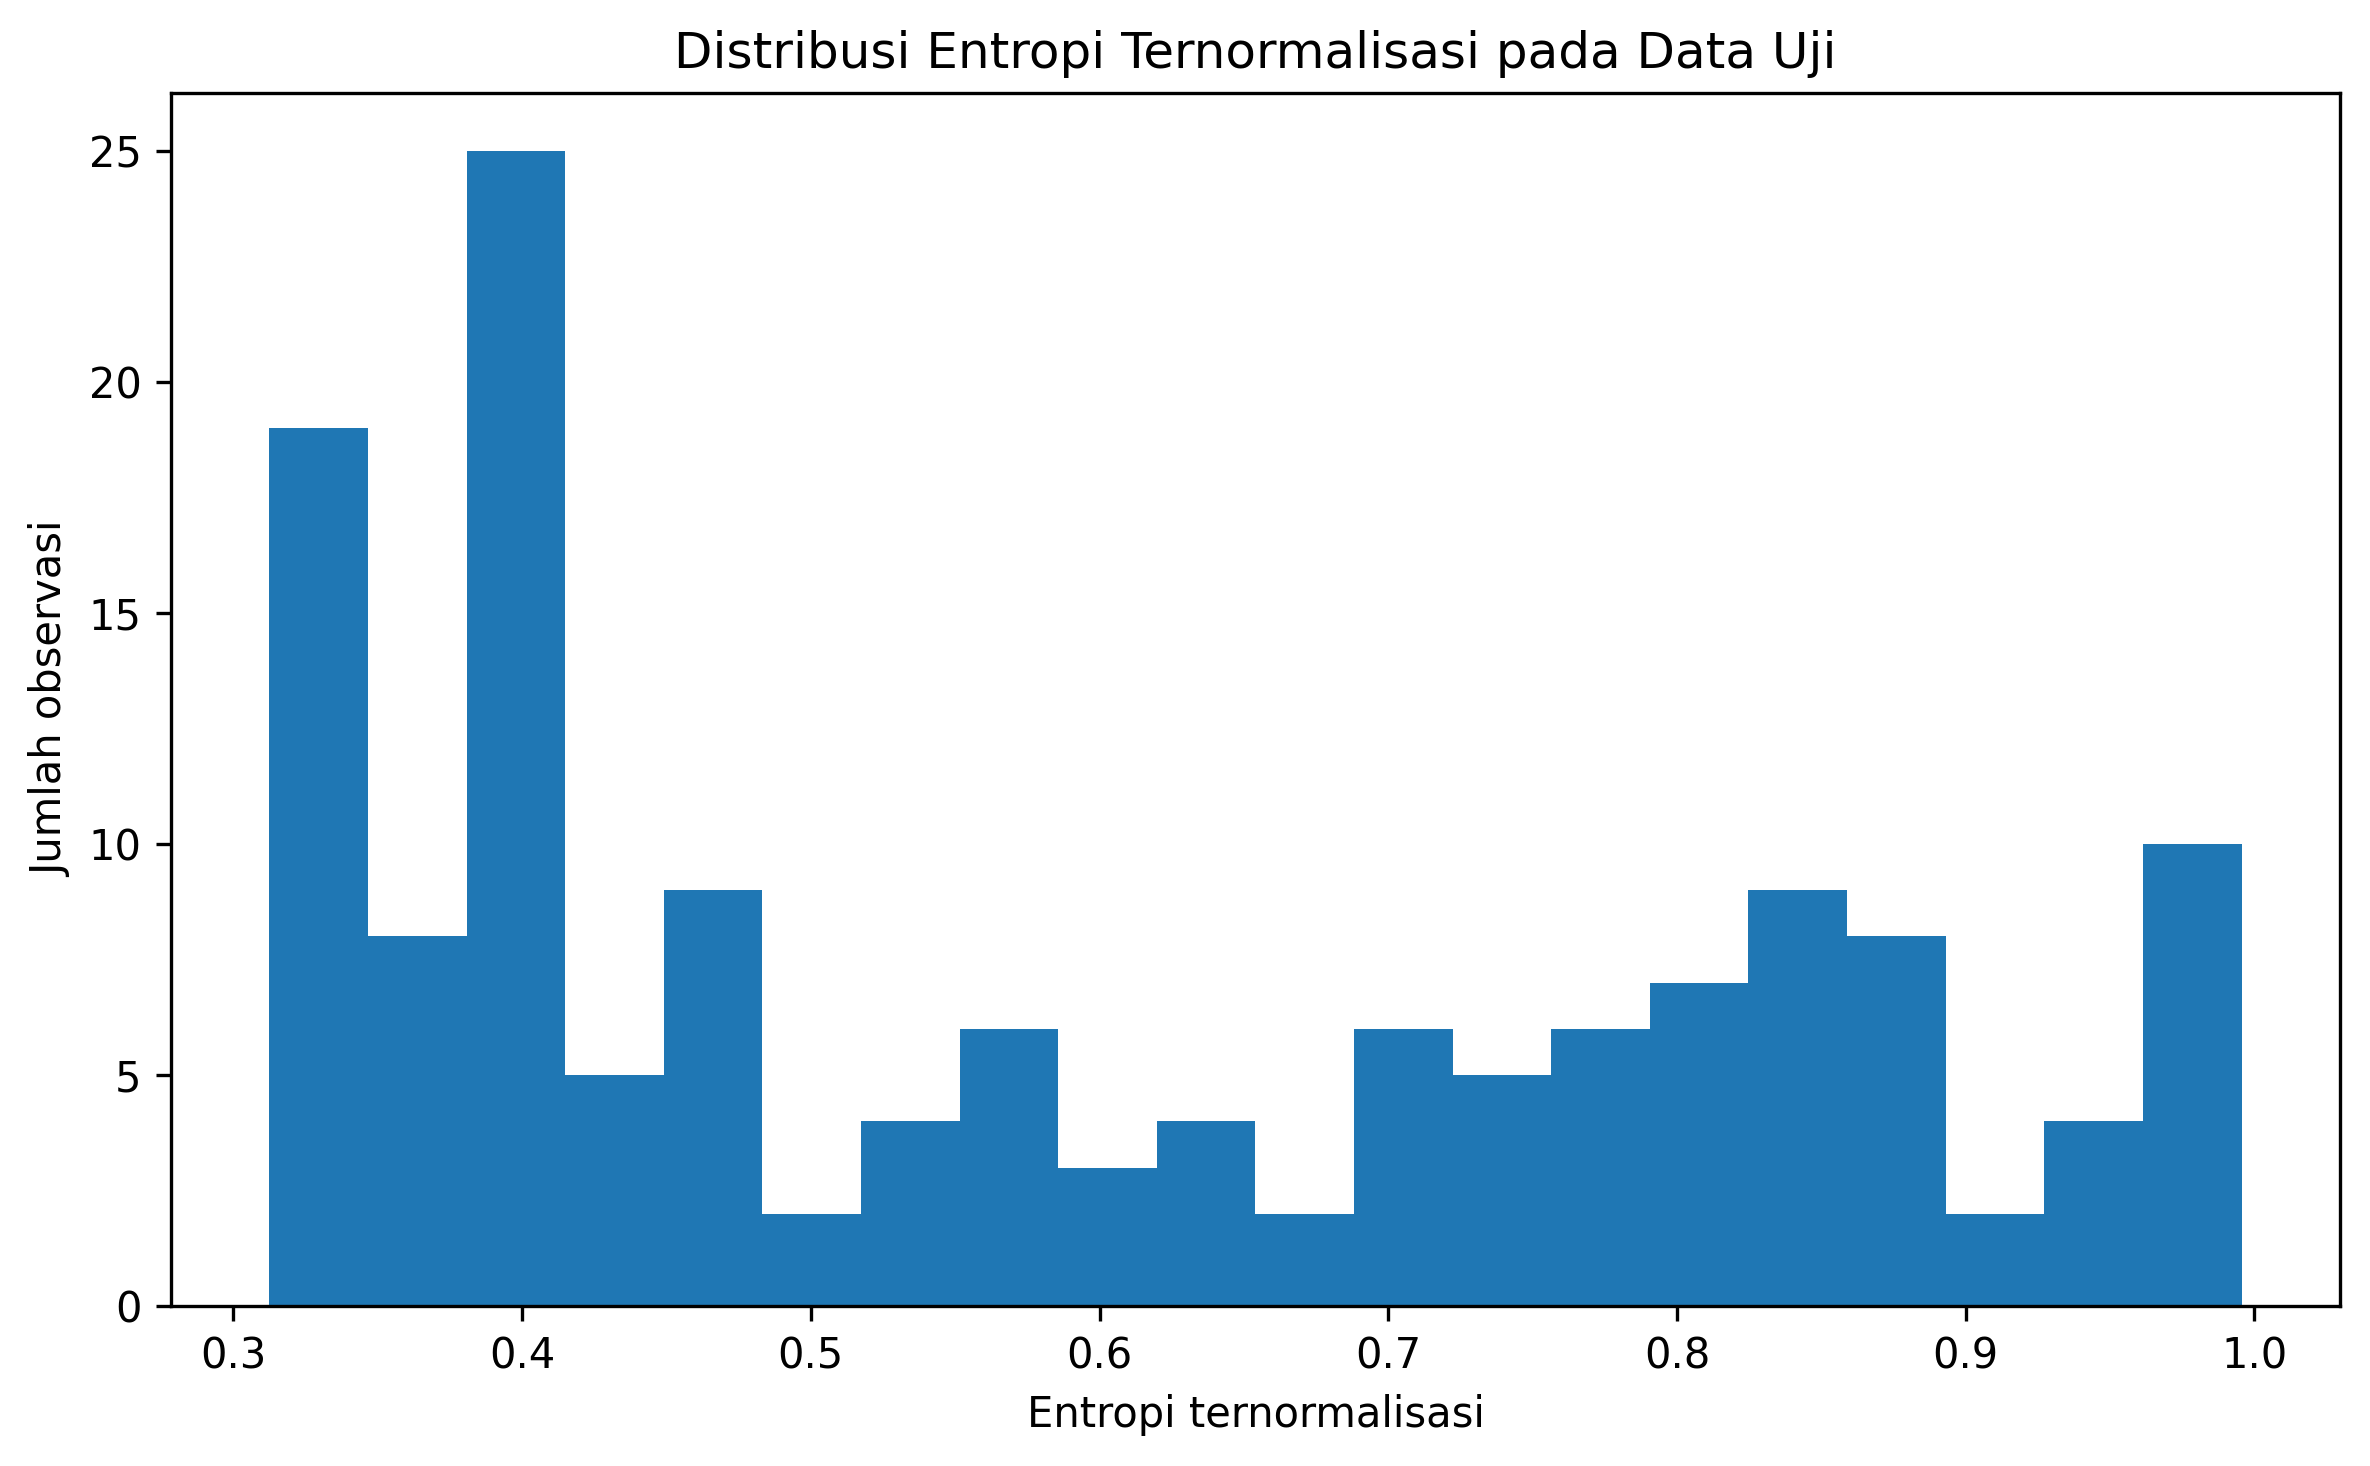
\includegraphics[width=0.85\textwidth]{normalized_entropy_distribution.png}
    \caption{TODO: sesuaikan caption untuk normalized_entropy_distribution.png}
    \label{fig:normalized_entropy_distribution}
\end{figure}

% shap_global_importance_top_features.png
\begin{figure}[!htbp]
    \centering
    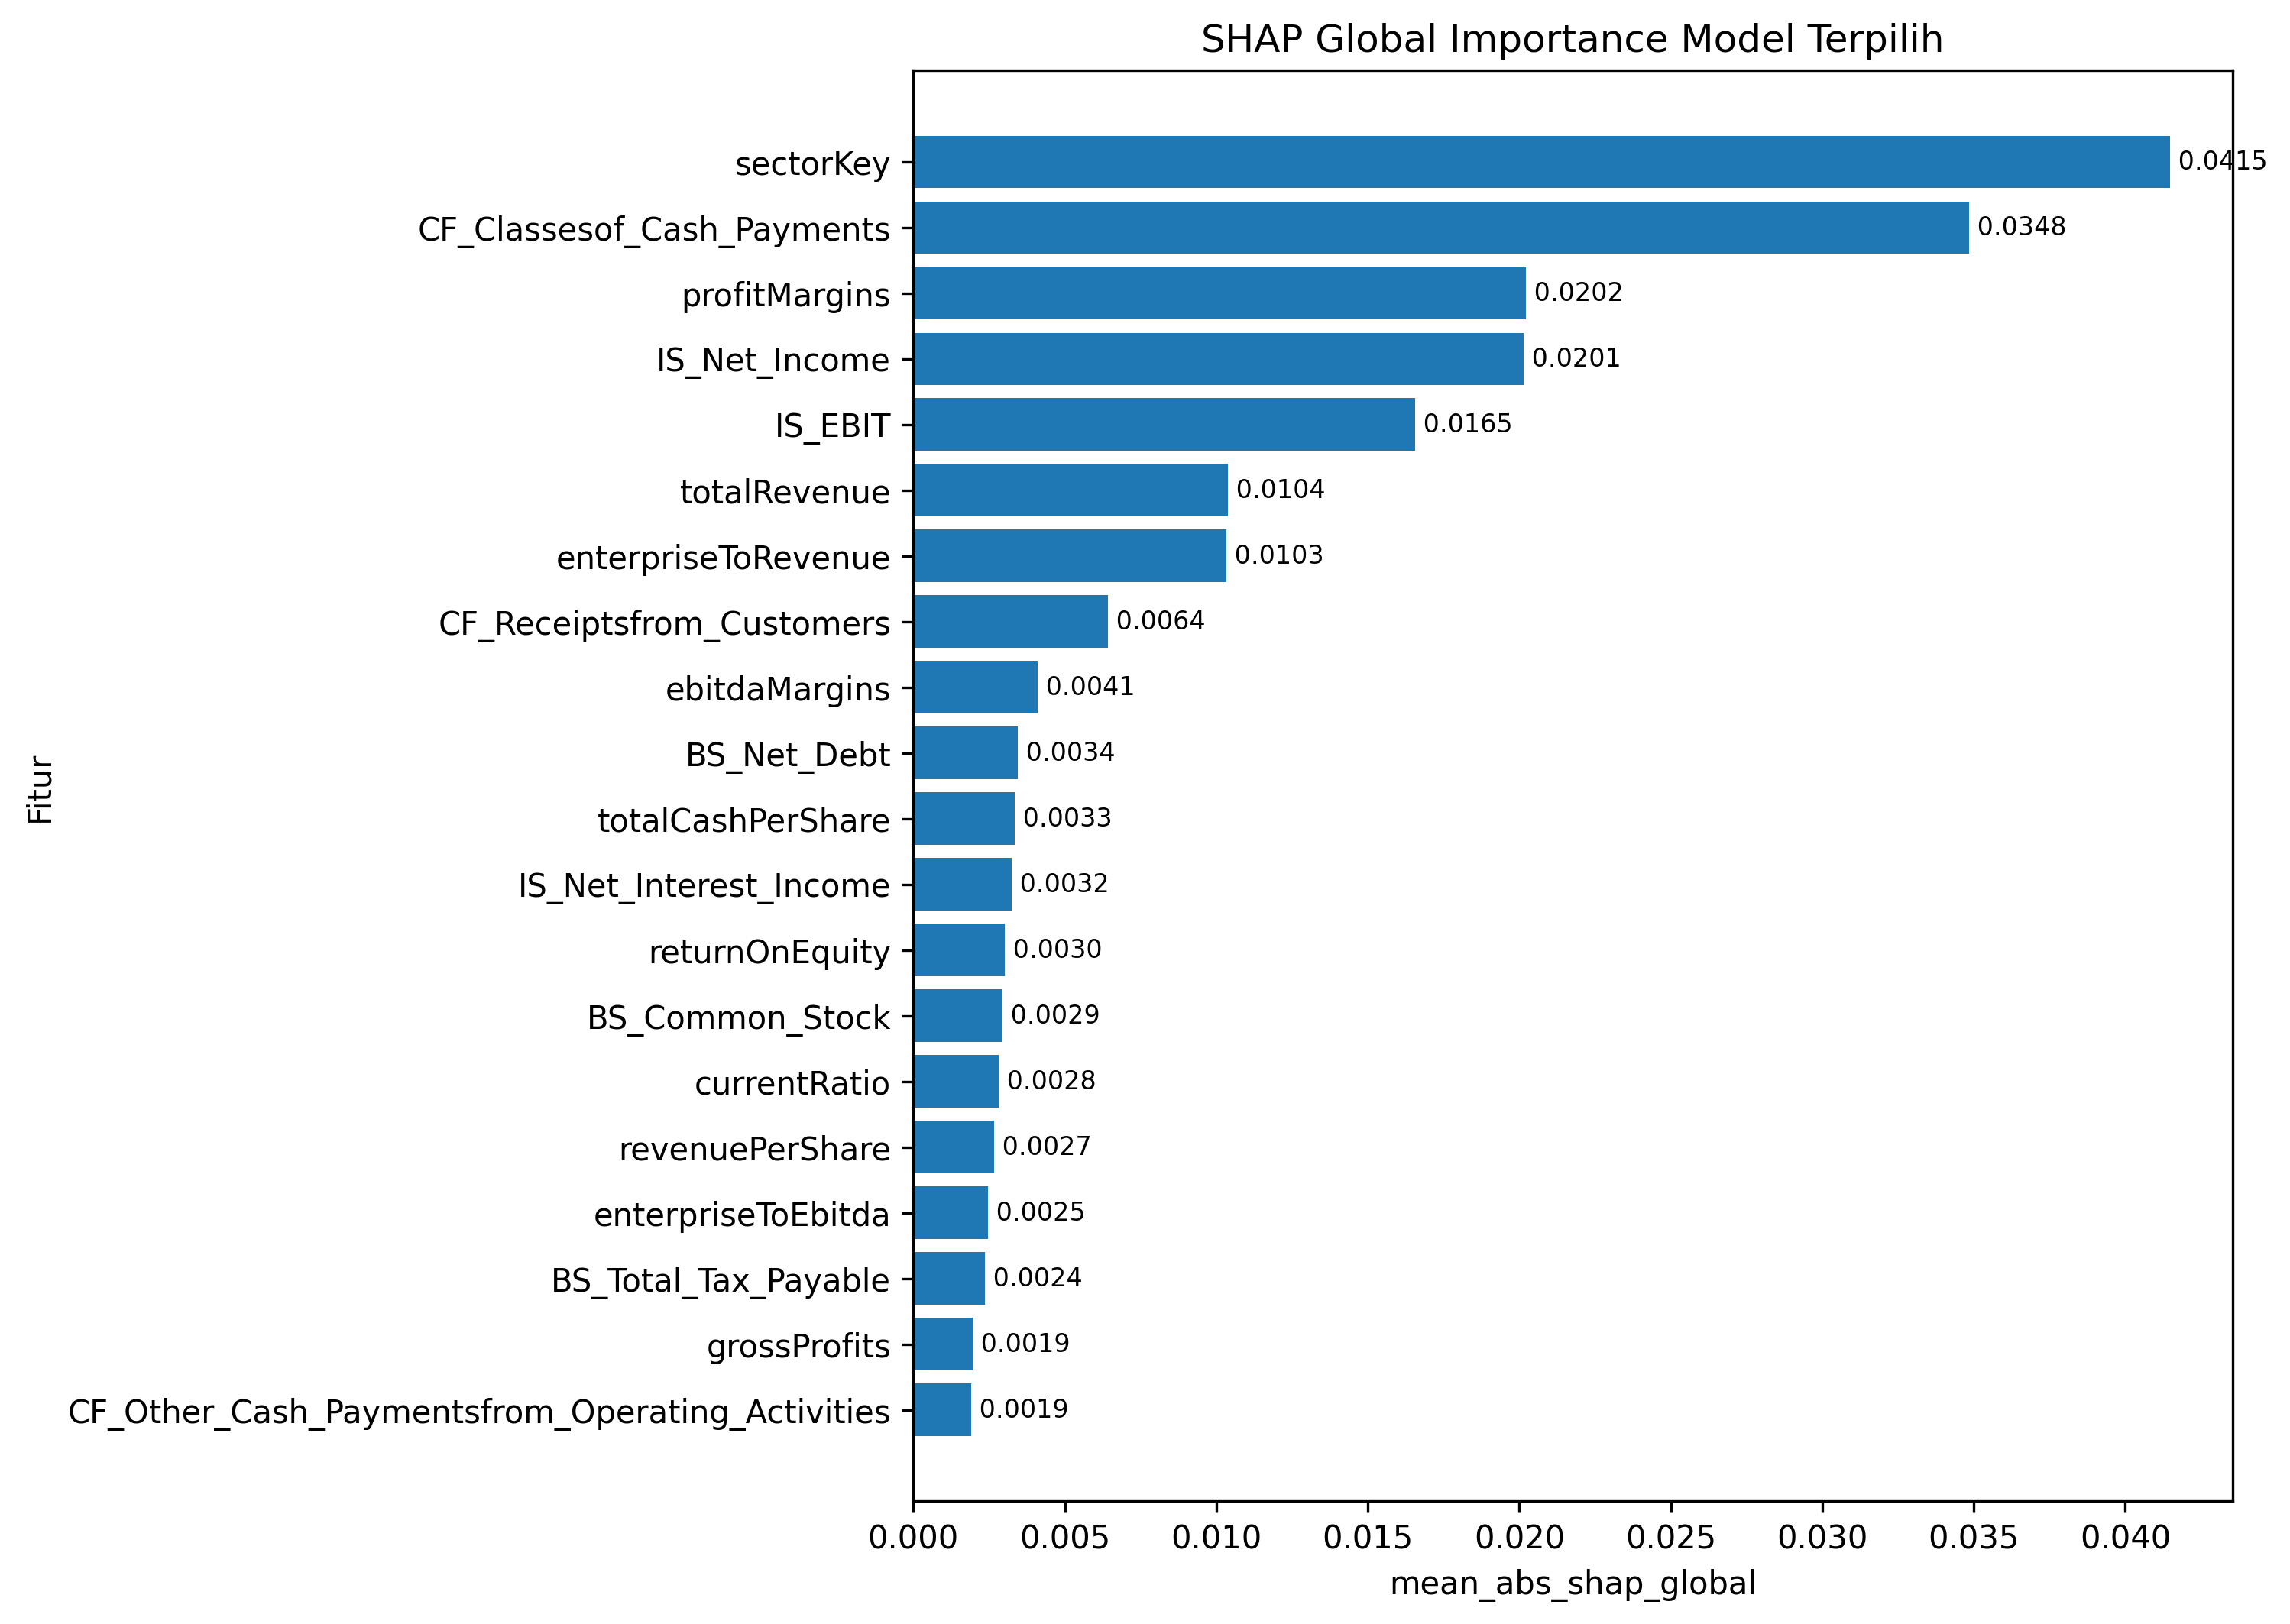
\includegraphics[width=0.85\textwidth]{shap_global_importance_top_features.png}
    \caption{TODO: sesuaikan caption untuk shap_global_importance_top_features.png}
    \label{fig:shap_global_importance_top_features}
\end{figure}

% rw_ucfi_global_importance_top_features.png
\begin{figure}[!htbp]
    \centering
    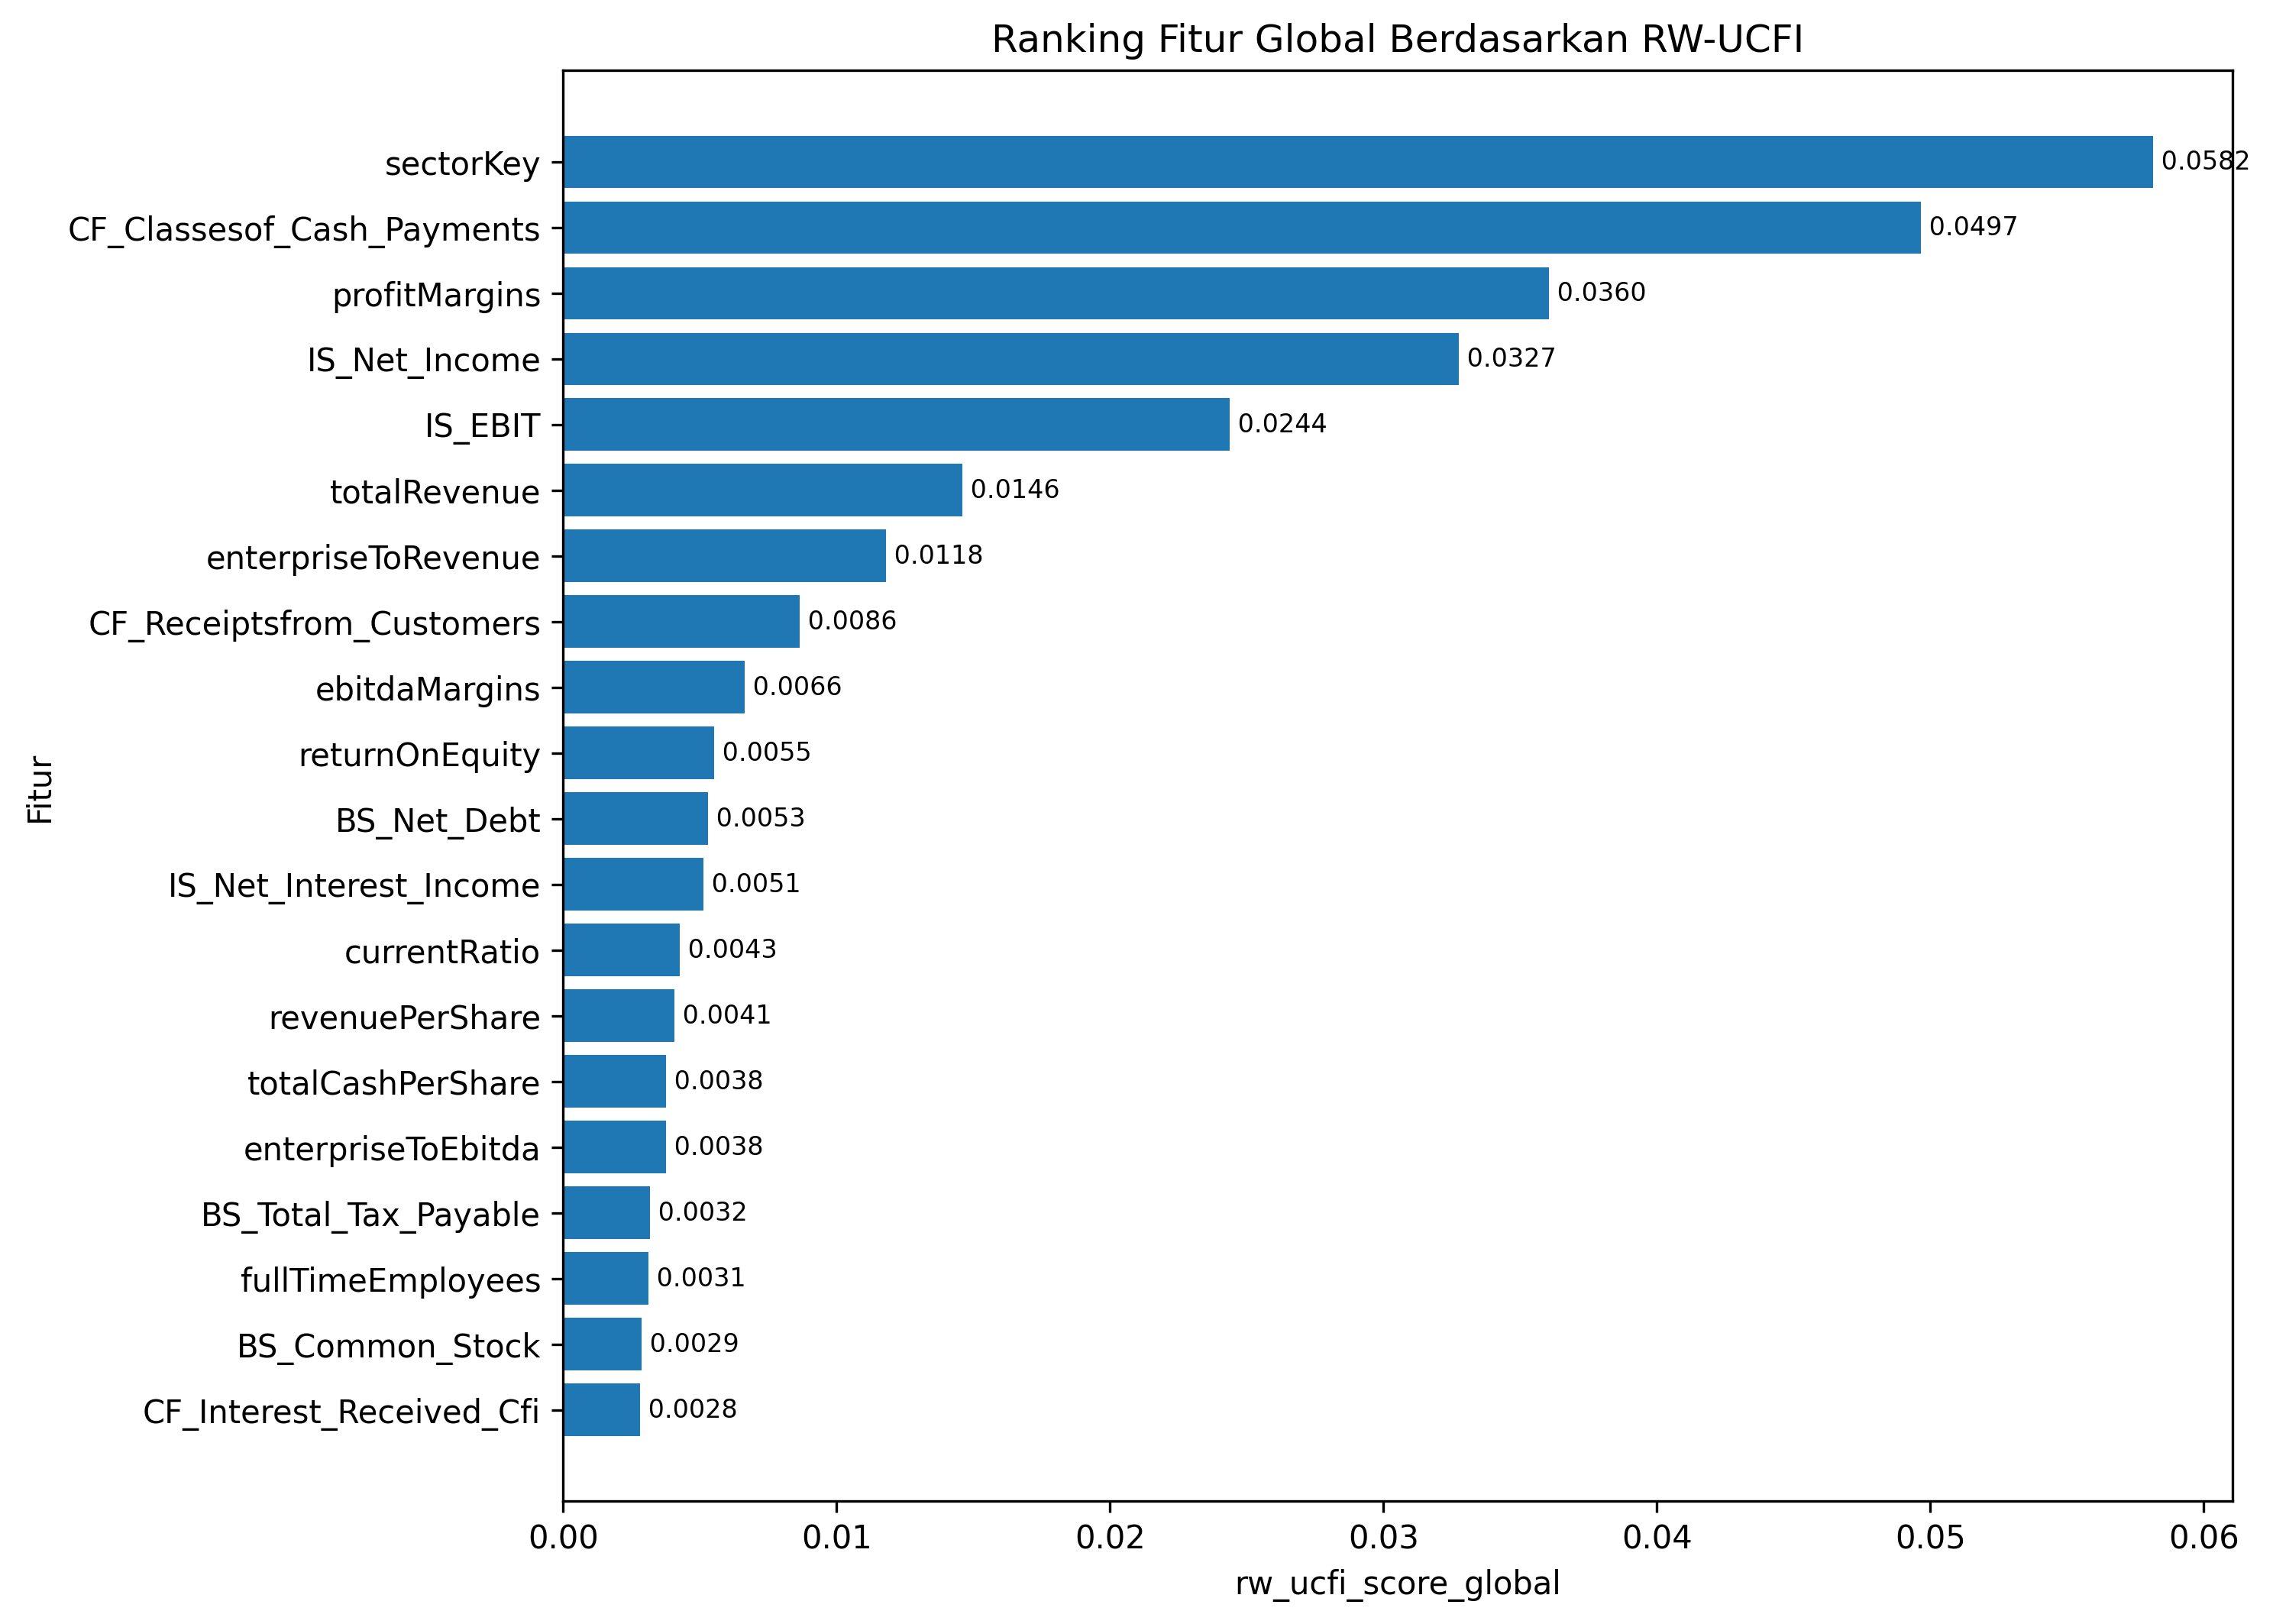
\includegraphics[width=0.85\textwidth]{rw_ucfi_global_importance_top_features.png}
    \caption{TODO: sesuaikan caption untuk rw_ucfi_global_importance_top_features.png}
    \label{fig:rw_ucfi_global_importance_top_features}
\end{figure}

% rw_ucfi_vs_shap_rank_shift_top_features.png
\begin{figure}[!htbp]
    \centering
    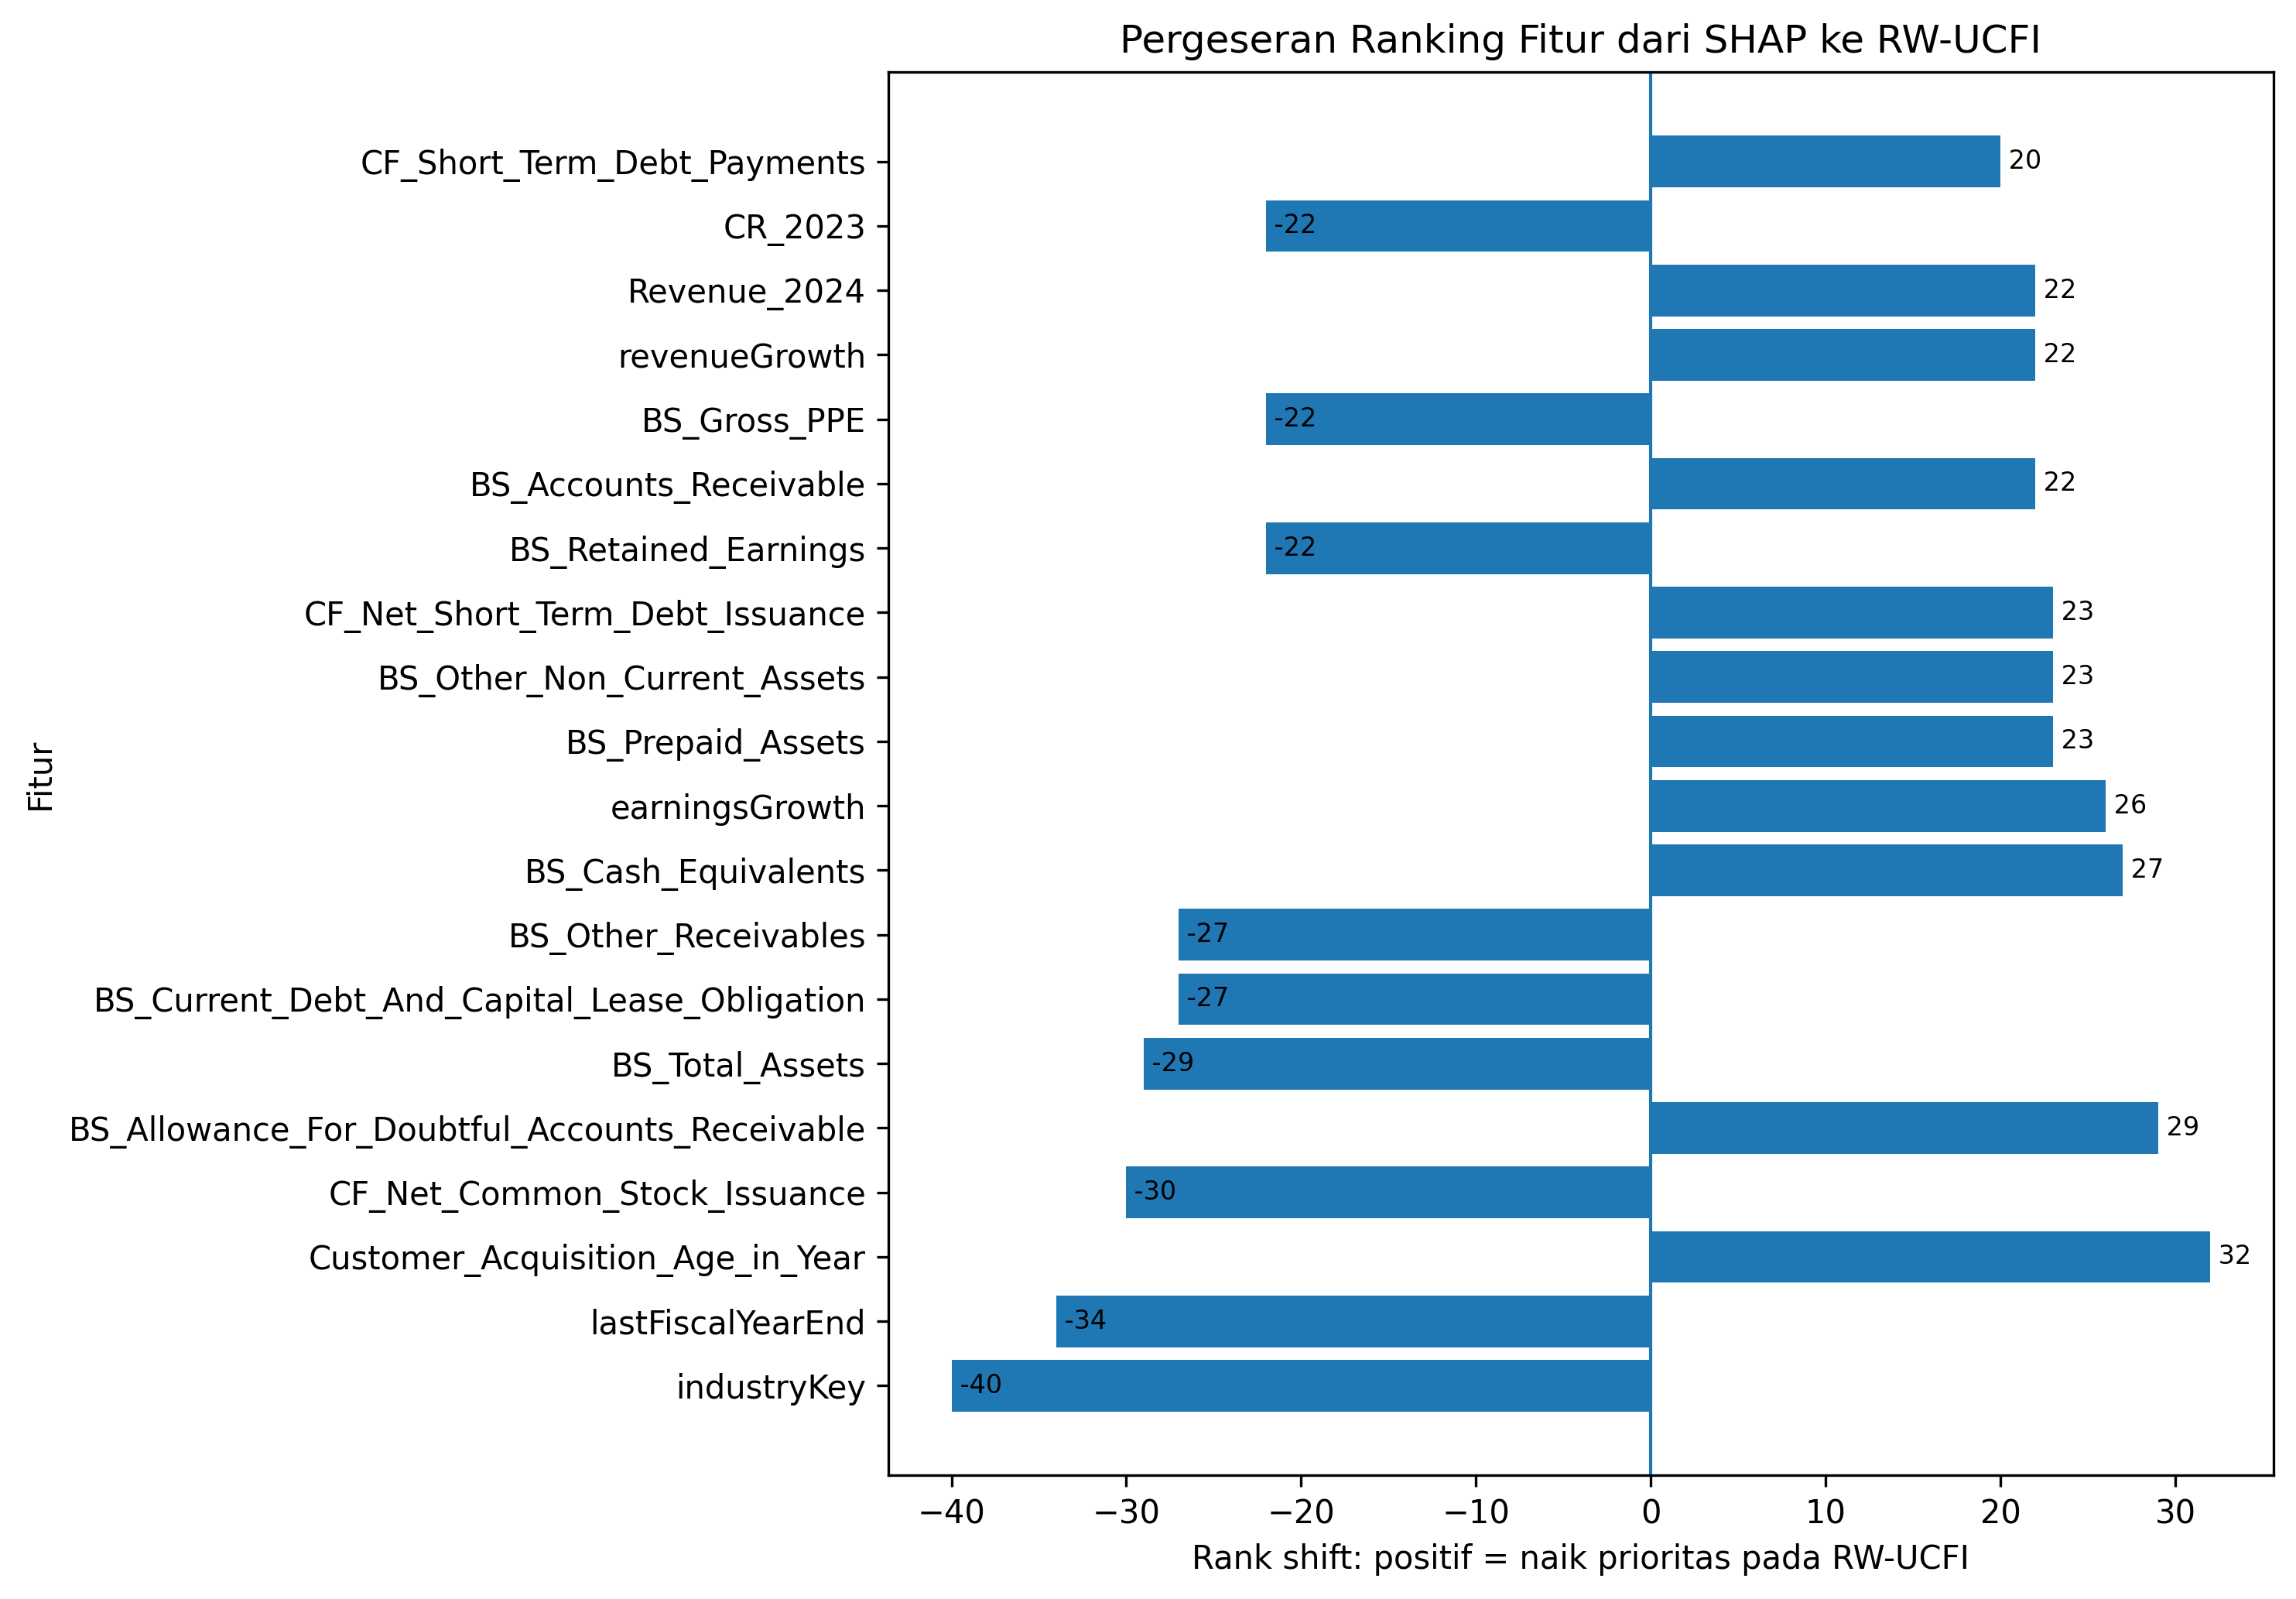
\includegraphics[width=0.85\textwidth]{rw_ucfi_vs_shap_rank_shift_top_features.png}
    \caption{TODO: sesuaikan caption untuk rw_ucfi_vs_shap_rank_shift_top_features.png}
    \label{fig:rw_ucfi_vs_shap_rank_shift_top_features}
\end{figure}

